% Copyright 2021 Joel Feldman, Andrew Rechnitzer and Elyse Yeager, except where noted.
% This work is licensed under a Creative Commons Attribution-NonCommercial-ShareAlike 4.0 International License.
% https://creativecommons.org/licenses/by-nc-sa/4.0/


%------------------------------------------------------
\section[1.8 Formal Limits at Infinity]{1.8 (Optional) Making Infinite Limits a Little More Formal}

 \begin{frame}{Table of Contents}
\begin{center}1.8 (Optional) Making Infinite Limits a Little More Formal\end{center}
\mapofcontentsA{}
 \end{frame}
%------------------------------------------------------
\note{One conceptual hurdle I've noticed with students is that the epsilon-delta definitions just have a lot of variables, and it's tough to remember which is which. I've had success in the past with the model below, I think because it disambiguates the parameters. Rather than an abstract list of variable names, it gives us a story with pieces that are easy to distinguish. ``The amount you put in the can," ``the amount your boss wants you to put in a can,"  ``the time you've been working," and ``the error in your can weight" are easier to keep straight then ``$f(x)$", ``$L$",  ``$x$," and ``$\epsilon$".
\\[1em]

Because limits at infinity have fewer moving parts (notably: you only have to worry about one ``side), I like to teach 1.8 \textit{before} 1.7.}
%------------------------------------------------------

\begin{frame}[t]
You work at a salmon cannery, putting salmon into cans. Each can is supposed to contain the amount of salmon shown on the label, but some error is allowable. As you work longer, and get more experience, the amount of error you are allowed to have gets smaller.
\vfill

\begin{tikzpicture}
%shrinking error margins
\onslide<2-4|handout:0>{
	\ycoord[C1]{1}{250}
	\ycoord[C1]{3}{750}}
\onslide<3-4|handout:0>{
	\draw[help lines] (0,1)--(9,1) (0,3)--(9,3);}
\onslide<4-4|handout:0>{
	\fill[W5] (1.1,1) rectangle (9.3,3)  (1,-.2) rectangle (1.4,-.7);}

\onslide<5-7|handout:0>{
	\ycoord[C1]{1.5}{375}
	\ycoord[C1]{2.5}{625}}
\onslide<6-7|handout:0>{
	\draw[help lines] (0,1.5)--(9,1.5) (0,2.5)--(9,2.5);}
\onslide<7-7|handout:0>{
	\fill[W5] (5.1,1.5) rectangle (9.3,2.5) (4.7,-.2) rectangle (5.3,-.7);
}


\onslide<8-10|handout:0>{
	\ycoord[C1]{1.6}{400}
	\ycoord[C1]{2.4}{600}}
\onslide<9-10|handout:0>{
	\draw[help lines] (0,1.6)--(9,1.6) (0,2.4)--(9,2.4);}
\onslide<10|handout:0>{
	\fill[W5] (7.1,1.6) rectangle (9.3,2.4) (7.2,-.2) rectangle (7.8,-.7);
}


%graph
\myaxis{t}{0}{9.25}{}{0}{3.5}
\ycoord{2}{500}
\foreach \x in {0,...,8}{
	\POWER{1.2}{-\x}{\a}
	\POWER{1.6}{-\x}{\b}
	\draw(\x+1,2+\a)node[]{
\includegraphics[width=2.5mm]{Clipart/can}};
	\draw(\x+0.5,2+\b)node[]{
\includegraphics[width=2.5mm]{Clipart/can}};
	\draw(\x+.25,2-\a)node[]{
\includegraphics[width=2.5mm]{Clipart/can}};
	\draw(\x+0.75,2-\b)node[]{
\includegraphics[width=2.5mm]{Clipart/can}};	
	}
\foreach \x in {1,...,36}{
	\xcoord{\x/4}{}}
\foreach \x in {5,10,...,35}{
	\xcoord{\x/4}{\x}}
\end{tikzpicture}
\index{
\includegraphics[height=5mm]{Clipart/can} ~\href{https://thenounproject.com/term/tuna-can/1453898/}{tuna can} by \href{https://thenounproject.com/throwawayicons/}{throwaway icons} is licensed under \CCBYthree}
\vfill

\color{C1}
\only<2-4>{Was there a time after which your error always \textit{less than} \alert{250} g?}
\only<5-7|handout:0>{Was there a time after which your error always \textit{less than} \alert{125} g?}
\only<8-10|handout:0>{Was there a time after which your error always \textit{less than} \alert{100} g?}
\note<3>{Emphasize: we don't really care exactly what that time was, we only need to know that it exists}
\note<6>{Good to point out that earlier, you were sometimes \textit{but not always} within the specified error tolerance. Non-monotone convergence is a common conceptual sticking point.}
\end{frame}

%------------------------------------------------------

\begin{frame}[t]
\AnswerSpace
\foreach \x in {1,...,5}{
	\MULTIPLY{\x}{2}{\A}
	\SUBTRACT{\A}{1}{\Q}
	\only<\Q>{\QuestionBar{\x}{5}\AnswerYes}
	\only<\A>{\AnswerBar{\x}{5}}
	}

Suppose the amount of salmon that is supposed to be in a can is 500 g. The amount of salmon you put into a can at time $x$ is $500+\frac6x$. 

\vfill

You need to reassure your boss that, after some time, your error is never more than \alert{\only<1-2>{3}\only<3-4|handout:0>{2}\only<5-6|handout:0>{1}\only<7-8|handout:0>{$\frac{1}{1000}$}\only<9-10|handout:0>{$\epsilon$} g}. Find such a time.
\vfill


\begin{tikzpicture}[xscale=0.75]%space to write on RHS
\myaxis{x}{0}{9.25}{}{0}{3.2}
\ycoord{1.5}{500}
\draw[dashed] (0,1.5)--(9,1.5);
\draw[double] (-.1,.5)--(.1,.5);
\draw[thick] plot[domain=0.5:9,smooth,samples=50]({\x},{1.25+1/(.2*\x+0.4)})node[above left]{$f(x)=500+\frac{6}{x}$};

	\color{W1}
	\onslide<2|handout:0>{\draw (0,2.5)-|(2,0);
		\ycoord{2.5}{503}
		\xcoord{2}{2}
	}
	\onslide<4|handout:0>{\draw (0,2.25)-|(3,0);
		\ycoord{2.25}{502}
		\xcoord{3}{3}
	}
	\onslide<6|handout:0>{\draw (0,1.875)-|(6,0);
		\ycoord{1.875}{501}
		\xcoord{6}{6}
	}

\end{tikzpicture}

\answer{\color{answercolor}
\foreach \s/\x/\y in {1/2/3,3/3/2,5/6/1,7/6000/\frac{1}{1000},9/\frac{6}{\epsilon}/\epsilon}{
	\ADD{\s}{1}{\ss}
\only<\s-\ss>{When $x > \onslide<\ss>{\x}$\quad then $|f(x)-500|< \y $.}
}}

\onslide<10>{No matter how exacting your boss is, if they give you a non-zero error allowance, you can \textit{always} schedule a time after which you will meet their standards.}
\end{frame}
%------------------------------------------------------
\begin{frame}[t]
\begin{block}{Definition~\eref{text}{def_1_8_1} (a)}
  Let $f$ be a function defined on the whole real line. We say that
\begin{quote}
  the limit as $x$ approaches $\infty$ of $f(x)$ is $L$
\end{quote}\\
and write
\begin{align*}
  \lim_{x \to \infty} f(x) &= L
\end{align*}
if and only if for every $\epsilon>0$ there exists $M \in \mathbb{R}$ so that
$|f(x)-L| < \epsilon$ whenever $x>M$.

Similarly we write
\begin{align*}
  \lim_{x \to -\infty} f(x) &= K
\end{align*}
if and only if for every $\epsilon>0$ there exists $N \in \mathbb{R}$ so that
$|f(x)-K| < \epsilon$ whenever $x<N$.


\end{block}
\end{frame}

%------------------------------------------------------

\begin{frame}
\begin{tabular}{p{0.5\textwidth} p{0.5\textwidth}}
\alert<1>{  Let $f$ be a function defined on the whole real line. } & \color{C1} $f(x)$:  actual can weights\\ \pause
%
\raggedright \alert<2>{ We say that
``the limit as $x$ approaches $\infty$ of $f(x)$ is $L$"
and write
\begin{align*}
  \lim_{x \to \infty} f(x) &= L
\end{align*}}& 
\color{C1} $L$: weight on the label that you want to match\\\pause
%
\alert<3>{if and only if for every $\epsilon>0$}
&
\color{C1} $\epsilon$: amount of allowable error
\\\pause
%
\raggedright\alert<4>{there exists $M \in \mathbb{R}$ so that
${|f(x)-L| < \epsilon}$ whenever $x>M$.}
&
\color{C1} $M$: time after which your weights are always off by less than $\epsilon$\\[1mm]
&\color{C1}$|f(x)-L|$: error  (difference between actual amount and label)
\end{tabular}\pause


\end{frame}

%------------------------------------------------------

\begin{frame}
\begin{tikzpicture}
\myaxis{x}{0}{8}{y}{0}{2}
\draw[thick] plot[domain=0:8,samples=100,smooth](\x,{1+0.75*sin(\x*5 r)*(1-\x/8.5)})node[right]{$y=f(x)$};
\onslide<2->{\ycoord{1}{L}}
\onslide<3-|handout:0>{
\color{W1}
\ycoord[above left]{1.2}{L+\epsilon}
\ycoord[below left]{0.8}{L-\epsilon}
\draw[dashed] (.2,1.2)--(8,1.2) (.2,0.8)--(8,0.8);
\onslide<4-|handout:0>{\xcoord{6.1}{M}}
}
\end{tikzpicture}
\vfill
\alert<1|handout:0>{  Let $f$ be a function defined on the whole real line. } \pause
 \alert<2|handout:0>{ We say that
``the limit as $x$ approaches $\infty$ of $f(x)$ is $L$"
and write
\begin{align*}
  \lim_{x \to \infty} f(x) &= L
\end{align*}}\pause
\alert<3|handout:0>{if and only if for every $\epsilon>0$} \pause
\alert<4|handout:0>{there exists $M \in \mathbb{R}$ so that
${|f(x)-L| < \epsilon}$ whenever $x>M$.}
\end{frame}

%------------------------------------------------------

\begin{frame}[t]
 \note<1>{For easy questions, students may wonder what the use of the definition is. Point out in later examples that it clears up ambiguity when the function is less obvious.}

\note<2>{Two things to note. One, that we have to find $M$, and that part is separate from the actual proof we write down. Two, we get to assume $x$ is large (so in this case, positive) because we only care about values larger than $M$. Remind students our cannery boss didn't care about our initial novice imprecision.}

\begin{block}{Definition~\eref{text}{def_1_8_1} (a)}
  Let $f$ be a function defined on the whole real line. We say that
$  \dlimx{\infty} f(x) = L$
if and only if for every $\epsilon>0$ there exists $M \in \mathbb{R}$ so that
$|f(x)-L| < \epsilon$ whenever $x>M$.
\end{block}
\color{C1}
\begin{QuestionSet}
\SetQuestion{%Q1
\AnswerYes
 Prove, using Definition \eref{text}{def_1_8_1}, that $\dlimx{\infty}\left[\frac2x+1\right] = 1$.}
\SetAnswer{\small
 Prove, using Definition \eref{text}{def_1_8_1}, that $\dlimx{\infty}\left[\frac2x+1\right] = 1$.\\
 \color{answercolor}
\begin{multicols}{2}Let $\epsilon$ be any positive constant. We need to find $M$ such that, for $x>M$:
\begin{align*}
\left|f(x)-L\right|&<\epsilon\\
\left|\left(\frac2x+1\right)-1\right|&<\epsilon\\
\left|\frac2x\right|&<\epsilon
\intertext{It suffices to find a positive $M$. Then $x$ is positive too.}
\frac2x&<\epsilon\\
x&>\frac2{\epsilon}
\end{align*}
So, we choose $M = \frac2{\epsilon}$. Now we can go through the definition.
\end{multicols}
}
\SetAnswer{
 Prove, using Definition \eref{text}{def_1_8_1}, that $\dlimx{\infty}\left[\frac2x+1\right] = 1$.\\\vfill
 \color{answercolor}
\textbf{Proof: }
Let $f(x) = \frac2x+1$. For any $\epsilon>0$, let $M = \frac{2}{\epsilon}$. Then for any $x>M$:
\begin{align*}
|f(x)-1|&=\left| \left(\frac2x+1\right)-1\right| = \left| \frac2x\right|=\frac2x\\
&<\frac2M = \frac{2}{\frac{2}{\epsilon}}=\epsilon
\end{align*}
Therefore $\dlimx{\infty}\left[\frac2x+1\right]=1$.\qed
}


%Q2
\SetQuestion{
\AnswerYes
  Prove, using Definition \eref{text}{def_1_8_1}, that  $\dlimx{\infty}\left[ 5e^{-x} \right]=0$}
\SetAnswer{
 Prove, using Definition \eref{text}{def_1_8_1}, that  $\dlimx{\infty}\left[ 5e^{-x} \right]=0$

 \color{answercolor}
 First, we need to find which $M$ goes with $\epsilon.$
 \begin{align*}
 |f(x)-L|&=\left| 5e^{-x}-0\right| = 5e^{-x}=
 \frac{5}{e^x}<\epsilon\\
 e^x &>\frac{5}{\epsilon}\\
 x&>\log_e\left(\frac5\epsilon\right)
 \end{align*}
 So, in our proof, we should use $M=\log_e\left(\frac5\epsilon\right)$
 }
 \SetAnswer{
 Prove, using Definition \eref{text}{def_1_8_1}, that  $\dlimx{\infty}\left[ 5e^{-x} \right]=0$

 \color{answercolor}
\textbf{Proof: } Set $f(x) = 5e^{-x}$. For any $\epsilon>0$, let $M = \log_e\left(\frac5\epsilon\right)$. Then for all $x$ that are greater than $M$:
\begin{align*}
\left| f(x)-0\right|&=\left| 5e^{-x}\right| = \frac{5}{e^x}\\
&<\frac{5}{e^M} = \frac{5}{e^{\log_e\left(\frac5e\right)}} = \frac{5}{\frac5\epsilon} = \epsilon
\end{align*}
Therefore, $\dlimx{\infty}[5e^{-x}]=0$. \qed
 }
 


%Q3
\SetQuestion{
\AnswerYes
\NowYou Prove, using Definition \eref{text}{def_1_8_1}, that   $\dlimx{\infty}\left[ \frac{\sin x}{x} \right]=0$
}
\SetAnswer{
 Prove, using Definition \eref{text}{def_1_8_1}, that   $\dlimx{\infty}\left[ \frac{\sin x}{x} \right]=0$

 \color{answercolor}
 \begin{multicols}{2}
 First, we find $M$ for an arbitrary $\epsilon$. We want
\[
|f(x) - 0|=\left|\frac{\sin x}{x}\right| < \epsilon
\]
We need to find values of $x$ that are large enough for this to be true, but we don't have to find the values of $x$ that make equality hold. (Think about the first canning example where we didn't even have numbers.) So, we simplify things by noting $|\sin x |<1$ for all $x$. For $x>0$,

 \begin{align*}
\left|\frac{\sin x}{x} \right|<\left| \frac1x\right| = \frac1x&<\epsilon\\
x&>\frac1\epsilon
 \end{align*}
 So, we use $M = \frac1\epsilon$.
\end{multicols}
 }\SetAnswer{
 Prove, using Definition \eref{text}{def_1_8_1}, that   $\dlimx{\infty}\left[ \frac{\sin x}{x} \right]=0$

 \color{answercolor}
\textbf{ Proof: }
Let $f(x) = \frac{\sin x}{x}$. For any $\epsilon>0$, let $M = \frac1\epsilon$. Whenever $x>M$:
\begin{align*}
\left| f(x)-0\right|&=\left| \frac{\sin x}{x}\right|\leq \left| \frac1x\right| = \frac1x\\
&<\frac1M = \epsilon
\end{align*}
So $\dlimx{\infty}\frac{\sin x}{x} = 0$. \qed
 }


%Q4
\SetQuestion{
\AnswerYes
\NowYou  Prove, using Definition \eref{text}{def_1_8_1}, that  $\dlimx{\infty}\left[\frac{2x^2}{x^2+1}\right]=2$ }
\SetAnswer{
Prove, using Definition \eref{text}{def_1_8_1}, that  $\dlimx{\infty}\left[\frac{2x^2}{x^2+1}\right]=2$ 

 \color{answercolor}

First, we find $M$ based on $\epsilon$.
\begin{align*}
\epsilon & >|f(x) - 2|=\left| \frac{2x^2}{x^2+1} - 2\right| = \left| \frac{2x^2-2(x^2+1)}{x^2+1}\right| = \left| \frac{-2}{x^2+1} \right|
=\frac{2}{x^2+1}\\
x^2+1&>\frac2\epsilon \implies x^2>\frac2\epsilon - 1
\implies x>\sqrt{\frac2\epsilon - 1}=M
\end{align*}
(If $\epsilon>2$, we can take $M=0$.)
Note that the values of $x$ that make $x^2>\frac2\epsilon - 1$ true are $(-\infty,-a) \cup (a,\infty)$ for $a=\sqrt{\frac2\epsilon - 1}$. Since we only care about large $x$, we use the second interval. (See graph on next slide.)
}
\SetAnswer{
 Prove, using Definition \eref{text}{def_1_8_1}, that  $\dlimx{\infty}\left[\frac{2x^2}{x^2+1}\right]=2$ 
\begin{tikzpicture}
\color{black}
\myaxis{x}{3}{3}{y}{0}{3}
\draw[C1, thick] plot[domain=-3:3](\x,{\x*\x/3})node[right]{$y=x^2$};
\draw[dashed] (-3,4/3)--(3,4/3)node[right]{$\frac{2}{\epsilon}-1$};
\xcoord{2}{\sqrt{\frac{2}{\epsilon}-1}}
\xcoord{-2}{-\sqrt{\frac{2}{\epsilon}-1}}
\end{tikzpicture}\hfill
\parbox[b]{.3\textwidth}{\color{answercolor}\raggedright
	It \textbf{is true} that for all $x>\sqrt{\frac2\epsilon-1}$, $x^2>\frac2\epsilon-1$.\\[1em]
	It \textbf{is not true} that for all $x>-\sqrt{\frac2\epsilon-1}$, $x^2>\frac2\epsilon-1$.\\[2em]}	
}
\SetAnswer{
 Prove, using Definition \eref{text}{def_1_8_1}, that  $\dlimx{\infty}\left[\frac{2x^2}{x^2+1}\right]=2$ 

 \color{answercolor}
\textbf{ Proof: }: Let $f(x) = \frac{2x^2}{x^2+1}$. 
For any $2\ge\epsilon>0$, set $M = \sqrt{\frac2\epsilon - 1}$. 
                (For $\epsilon>2$, set $M=0$.)
                Then for any $x>M$:
\begin{align*}
|f(x) - 2| &=\left| \tfrac{2x^2}{x^2+1}-2 \right| = \left|\tfrac{-2}{x^2+1}\right| = \tfrac{2}{x^2+1}\\
&<\frac2{M^2+1} = \tfrac{2}{\left(\sqrt{\frac2\epsilon - 1}\right)^2+1} = \frac{2}{\frac2\epsilon-1+1}=\epsilon
\end{align*}
So $\dlimx{\infty}\left[\frac{2x^2}{x^2+1}\right]=2$.\qed
}


%Q5
\SetQuestion{
\AnswerYes
 Prove, using Definition \eref{text}{def_1_8_1}, that  $\dlimx{\infty} 5 = 5$
 }
\SetAnswer{
 Prove, using Definition \eref{text}{def_1_8_1}, that  $\dlimx{\infty} 5 = 5$

 \color{answercolor}
\textbf{ Proof: }: Let $f(x) = 5$, and let $M=1$. For any $\epsilon >0$, and for any $x>M$:
 \begin{align*}
 |f(x)-5| = 5-5 = 0 < \epsilon
 \end{align*}
 So, $\dlimx{\infty} 5 = 5$. \qed \\ \vfill
 Note: you actually could have chosen \textit{any} value for $M$.
 }


%Q6
\SetQuestion{
\AnswerYes
True or False? $\dlimx{\infty} \sin x = 0$
 }
\SetAnswer{
True or False? $\dlimx{\infty} \sin x = 0$

 \color{answercolor}
False.

Let $f(x)=\sin x$ and consider $\epsilon = \frac12$. Note that when $x=\frac{\pi}{2}+n\pi$ for any integer $n$, then $\sin x = \pm 1$, so
\[|f(x)-0| = |\pm 1|=1>\frac12\]
So there is \textit{no} point after which $f(x)$ is always within $\frac12$ of $0$. Therefore $\dlimx{\infty} \sin x \neq 0$.
 }
\SetAnswer{
True or False? $\dlimx{\infty} \sin x = 0$
\color{black}
\begin{tikzpicture}
\myaxis{x}{0}{8}{y}{1}{1}
\draw[C1, thick] plot[domain=0:8,smooth,samples=50](\x,{sin(3*\x r)})node[right]{$y=\sin x$};
\ycoord{.5}{0+\frac12}
\ycoord{-.5}{0-\frac12}
\draw[dashed] (.2,.5)--(8,.5) (.2,-.5)--(8,-.5);
\end{tikzpicture}
 }
 



 \end{QuestionSet}
\end{frame}

%------------------------------------------------------

\begin{frame}[t]{Useful General Principles}
When we showed $\dlimx{\infty}\left[\frac{\sin x}{x}\right]=0$, we chose $M$ using:
\[\left|\frac{\sin x}{x}\right|\le \left| \frac1x\right| = \frac1x<\epsilon\]
\pause
\begin{itemize}[<+->]
\item $\left|\frac1x\right|=\frac1x$ only when $x$ is positive. We want to show that an inequality holds for \textit{large enough} values of $x$, so if it helps our cause, we can say ``make sure $x$ is larger than \textit{blah}." Then we just choose $M$ to be at least that number \textit{blah}.
\item If $a<b<c$, then $a<c$. So if you want to solve $a<c$, but it's too hard to find \textit{exactly} when that's true, see whether you can replace $a$ with a larger, easier expression $b$.

That's what we did when we said $\left|\frac{\sin x}{x}\right| \le \left| \frac1x\right|$.
\end{itemize}
\end{frame}

%------------------------------------------------------

%------------------------------------------------------

\begin{frame}[t]{Limit as $x$ goes to negative infinity}
\AnswerSpace
\only<2>{\AnswerYes\MoreSpace\QuestionBar{1}{2}}
\begin{block}{Definition~\eref{text}{def_1_8_1} (a)}
We write
\begin{align*}
  \lim_{x \to -\infty} f(x) &= K
\end{align*}
if and only if for every $\epsilon>0$ there exists $N \in \mathbb{R}$ so that
$|f(x)-K| < \epsilon$ whenever $x<N$.
\end{block}\pause
\textcolor{C1}{Use Definition~\eref{text}{def_1_8_1} to prove $\dlimx{-\infty}\frac{x^3}{x^3+1}=1$}
\end{frame}
%------------------------------------------------------------------
\begin{frame}<beamer>[t]
\only<1>{\QuestionBar{1}{2}\AnswerYes}
\only<2->{\AnswerBar{1}{2}}
\textcolor{C1}{Use Definition~\eref{text}{def_1_8_1} to prove $\dlimx{-\infty}\frac{x^3}{x^3+1}=1$}\pause

\color{answercolor}
\only<2>{
Let $f(x) = \frac{x^3}{x^3+1}$ and $\epsilon>0$.
\begin{multicols}{2}
Since we are now concerned with highly \textit{negative} values of $x$, we can assume that $x$ is a large negative number.

To find $N$, we solve the inequality:
\begin{align*}
\epsilon &>|f(x)-1| = \left| \frac{x^3}{x^3+1}-1\right|\\
&=\left|\frac{x^3}{x^3+1} - \frac{x^3+1}{x^3+1} \right|\\
&=\left|\frac{-1}{x^3+1}\right|
\intertext{Since we will be choosing highly negative values of $x$, the denominator $x^3+1$ is a negative number. Then $\frac{-1}{x^3+1}$ is a positive number.}
&=\frac{-1}{x^3+1}
\intertext{So we have}
\epsilon&>\frac{-1}{x^3+1}
\end{align*}
\end{multicols}
}
\only<3>{\color{answercolor}
\begin{align*}
\epsilon&>\frac{-1}{x^3+1}
\intertext{The denominator is negative, so when we multiply both sides by it, we flip the inequality}
\epsilon(x^3+1)&<-1\\
\epsilon x^3 + \epsilon &<-1\\
\epsilon x^3 &<-1-\epsilon\\
x^3&<\frac{-1-\epsilon}{\epsilon} = -\left(1+\frac{1}{\epsilon}\right)\\
x&< -\left(1+\frac{1}{\epsilon}\right)^{1/3}
\end{align*}
Choose $N = -\left(1+\frac1\epsilon\right)^{1/3}$.}
\only<4>{
\textbf{ Proof: }: 
Set $f(x) = \frac{x^3}{x^3+1}$. For any $\epsilon>0$, let $N = -\left(1+\frac1\epsilon\right)^{1/3} $. Then for any $x<N$:
\begin{align*}
|f(x)-1|&=\left|  \frac{x^3}{x^3+1} - 1 \right| = \left| \frac{-1}{x^3+1}\right|= \frac{-1}{x^3+1}\\
&<\frac{-1}{N^3+1} =\frac{-1}{\left( -\left(1+\frac1\epsilon\right)^{1/3} \right)^3+1}  
=\frac{-1}{-(1+\frac1\epsilon)+1} \\
&=\frac{-1}{-\frac1\epsilon} = \epsilon
\end{align*}
So, $\dlimx{-\infty} \frac{x^3}{x^3+1}=1$.\qed
}
\end{frame}
%------------------------------------------------------------------

%------------------------------------------------------

\begin{frame}[t]{Limit as $x$ goes to negative infinity}
\AnswerYes\MoreSpace\QuestionBar{2}{2}
\begin{block}{Definition~\eref{text}{def_1_8_1} (a)}
We write
\begin{align*}
  \lim_{x \to -\infty} f(x) &= K
\end{align*}
if and only if for every $\epsilon>0$ there exists $N \in \mathbb{R}$ so that
$|f(x)-K| < \epsilon$ whenever $x<N$.
\end{block}
\textcolor{C1}{Use Definition~\eref{text}{def_1_8_1} to prove $\dlimx{-\infty}\frac{\cos x}{\sqrt{x^4+x^2+1}}=0$}
\end{frame}
%----------------------------------------------------------------------------------------
\begin{frame}<beamer>[t]
\only<1>{\AnswerYes \QuestionBar{2}{2}}
\only<2->{\AnswerBar{2}{2}}
\textcolor{C1}{Use Definition~\eref{text}{def_1_8_1} to prove $\dlimx{-\infty}\frac{\cos x}{\sqrt{x^4+x^2+1}}=0$\\}\pause\color{answercolor}
\only<2>{
Let's start by getting a handle on the inequality we know we'll be solving:
\[
\epsilon>|f(x)-0| = \left|\frac{\cos x}{\sqrt{x^4+x^2+1}}\right| = \frac{|\cos x|}{\sqrt{x^4+x^2+1}}
\]
We've seen something similar with sine. Since $|\cos x|\le1$, we can solve instead the right-most inequality below:
\[ \frac{|\cos x|}{\sqrt{x^4+x^2+1}}\le \frac{1}{\sqrt{x^4+x^2+1}}< \epsilon\]
But why stop there? Let's solve the right-most inequality below:
\begin{align*} \frac{|\cos x|}{\sqrt{x^4+x^2+1}}\le \frac{1}{\sqrt{x^4+x^2+1}}
 < \frac{1}{\sqrt{x^4}} = \frac{1}{x^2}
< \epsilon
 \end{align*}
 So, we set $N =- \frac{1}{\sqrt \epsilon}$. (Note $\frac{1}{x^2}$ is \textit{not} always less than $\epsilon$ if $x$ only has to be less than $\frac{1}{\sqrt \epsilon}$. A graph can help explain this -- see next slide.)}
 \only<3>{
 \vfill
\begin{tikzpicture}
\color{black}
\myaxis{x}{3}{3}{y}{0}{3}
\draw[C1, thick] plot[domain=0.58:3](\x,{1/(\x*\x)})node[above]{$y=\frac{1}{x^2}$};
\draw[C1, thick] plot[domain=-0.58:-3](\x,{1/(\x*\x)});
\draw[dashed] (-3,1)--(3,1)node[right]{$\epsilon$};
\xcoord{1}{\frac{1}{\sqrt \epsilon}}
\xcoord{-1}{-\frac{1}{\sqrt \epsilon}}
\end{tikzpicture}\hfill
\parbox[b]{.3\textwidth}{\color{answercolor}\raggedright
	It \textbf{is true} that for all $x<-\frac{1}{\sqrt\epsilon}$, $\frac{1}{x^2}<\epsilon$.\\[1em]
	It \textbf{is not true} that for all $x<\frac{1}{\sqrt\epsilon}$, $\frac{1}{x^2}<\epsilon$.\\[2em]}	 
	\vfill

We want to find $N$ that guarantees that $\frac{1}{x^2}<\epsilon$ 
whenever $x<N$. That's why we choose $N=-\frac{1}{\sqrt \epsilon}$.

Now we're ready to start our proof.
}
 \only<4>{
 \vfill
\textbf{ Proof: }: Let $f(x) = \frac{\cos x}{\sqrt{x^4+x^2+1}}$. For any $\epsilon>0$, set $N=- \frac{1}{\sqrt \epsilon}$. Then for any $x<N$:
 \begin{align*}
 |f(x)-0|&=\frac{|\cos x|}{\sqrt{x^4+x^2+1}} < \frac{1}{x^2}\\
\intertext{Note that $x<N<0$, so $|x|>|N|$ and $x^2>N^2$. Then:}
|f(x)-0|<\frac{1}{x^2}&<\frac{1}{N^2} = \frac{1}{\left( -\frac{1}{\sqrt \epsilon}\right)^2} = \epsilon
 \end{align*}
 So, $\dlimx{-\infty}\frac{\cos x}{\sqrt{x^4+x^2+1}}=0$.\qed
 \vfill
 }
\end{frame}
%----------------------------------------------------------------------------------------

%------------------------------------------------------

\begin{frame}[t]{Infinite Limits}
\begin{block}{Definition~\eref{text}{def_1_8_1} (c)}
Let $f$ be a function defined on the whole real line. We write
\[\lim_{x \to \infty}f(x)=\infty\]
if and only if for every \alert<2|handout:0>{$P>0$} there exists \alert<3|handout:0>{$M>0$} so that \alert<4|handout:0>{$f(x)>P$ whenever $x>M$}.
\end{block}
\begin{center}\begin{tikzpicture}
\myaxis{x}{0}{6}{y}{0}{2}
\onslide<2-|handout:0>{\ycoord{1}{\alert<2>{P}} \draw[dashed] (.2,1)--(6,1);}
\onslide<3-|handout:0>{\xcoord{5.3}{\alert<3>{M}}}
\onslide<4-|handout:0>{\draw[M5,line width=4pt] plot[domain=5.3:6,smooth](\x,{exp(\x)/200});}
\draw[C1, thick] plot[domain=0:6,smooth](\x,{exp(\x)/200});
\end{tikzpicture}\end{center}
\end{frame}

%------------------------------------------------------

\begin{frame}[t]
\AnswerSpace
\foreach \n in {1,2,3,4}{
	\MULTIPLY{\n}{2}{\q}
	\ADD{\q}{1}{\a}
	\only<\q>{\QuestionBar{\n}{4}\AnswerYes}
	\only<\a>{\AnswerBar{\n}{4}}
	}
\begin{block}{Definition~\eref{text}{def_1_8_1} (c)}
Let $f$ be a function defined on the whole real line. We write
$\dlimx{\infty}f(x)=\infty$
if and only if for every $P>0$ there exists $M>0$ so that $f(x)>P$ whenever $x>M$.
\end{block}
\begin{multicols}{2}
\begin{tikzpicture}
\myaxis{x}{0}{4}{y}{0}{4}

\onslide<2-3|handout:0>{

\ycoord{1}{1} \draw[dashed] (.2,1)--(4,1);}
\onslide<3|handout:0>{\xcoord{2}{2}
\draw[M5,line width=4pt] plot[domain=2:4,smooth](\x,{\x*\x/4});
}

\onslide<4-5|handout:0>{\ycoord{2}{2} \draw[dashed] (.2,2)--(4,2);}
\onslide<5|handout:0>{\xcoord{2.83}{\sqrt 8}
\draw[M5,line width=4pt] plot[domain=2.83:4,smooth](\x,{\x*\x/4});
}

\draw[C1, thick] plot[domain=0:4,smooth](\x,{\x*\x/4})node[left,xshift=-1mm]{$f(x)=\frac{x^2}{4}$};
\end{tikzpicture}
\columnbreak
\pause

Let \only<2-3>{$P=1$}\only<4-5>{$P=2$}\only<6-7>{$P=1\, 000\, 000$}\only<8-9>{$P>0$}. Find $M>0$ so that $f(x)>P$ whenever $x>M$.

\only<3|handout:0>{\textcolor{answercolor}{\begin{align*}
1&<\frac{x^2}{4}\\
4&<x^2\\
2&<x
\end{align*}}}
\only<5|handout:0>{\textcolor{answercolor}{\begin{align*}
2&<\frac{x^2}{4}\\
8&<x^2\\
\sqrt 8&<x
\end{align*}}}
\only<7|handout:0>{\textcolor{answercolor}{\begin{align*}
10^6&<\frac{x^2}{4}\\
4\times 10^6&<x^2\\
2\times 10^3&<x
\end{align*}}}
\only<9|handout:0>{\textcolor{answercolor}{\begin{align*}
P&<\frac{x^2}{4}\\
4P&<x^2\\
2\sqrt P&<x
\end{align*}}}
\end{multicols}
\end{frame}

%------------------------------------------------------
%------------------------------------------------------

\begin{frame}[t]
\begin{block}{Definition~\eref{text}{def_1_8_1} (c)}
Let $f$ be a function defined on the whole real line. We write
$\dlimx{\infty}f(x)=\infty$
if and only if for every $P>0$ there exists $M>0$ so that $f(x)>P$ whenever $x>M$.
\end{block}
\begin{QuestionSet}
%Q1
\SetQuestion{Using definition~\eref{text}{def_1_8_1}, prove or disprove the following:
\[\dlimx{\infty}  \sqrt[3] x = \infty\]}
\SetAnswer{Using definition~\eref{text}{def_1_8_1}, prove or disprove the following:
\[\dlimx{\infty}  \sqrt[3] x = \infty\]
\color{answercolor}
Let $P>0$ and $f(x) = \sqrt[3]{x}$. We should find a value of $M$ so that $f(x)>P$ whenever $x>M$.
\begin{align*}
P&<f(x) = x^{1/3}\\
P^3&<x
\end{align*}
So, we choose $M=P^3$.\vfill

\textbf{Proof:} For any $P>0$, let $M=P^3$. Then whenever $x>M$,  $\sqrt[3]{x}>\sqrt[3]{M} =\sqrt[3]{P^3}=P $. So, $\dlimx{\infty}\sqrt[3]{x}=\infty$.
}


%Q2
\SetQuestion{Using definition~\eref{text}{def_1_8_1}, prove or disprove the following:
\[\dlimx{\infty} x(\sin x + 1) = \infty\]}
\SetAnswer{Using definition~\eref{text}{def_1_8_1}, prove or disprove the following:
\[\dlimx{\infty} x(\sin x + 1) = \infty\]\color{answercolor}
Let $f(x) = x(\sin x + 1)$. Note that when $x = (2n+1.5)\pi$ for any integer $n$ (e.g. $x=\frac32\pi$, $x=\frac72\pi$, $x=\frac{11}{2}\pi$), then $f(x) = x(-1+1)=0$. So even if we narrow our focus to very large values of $x$, there will always be a value of $x$ where $f(x) = 0$. That tells us that the statement is not true, and gives us the examples we need to disprove it.
}
\SetAnswer{
\vfill
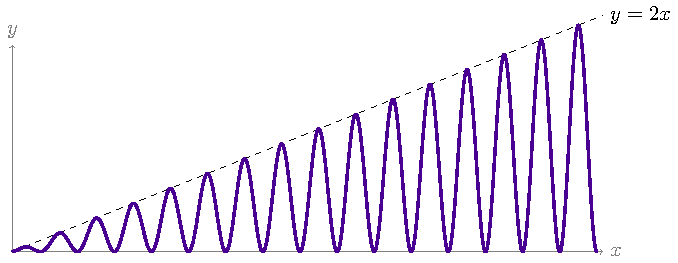
\includegraphics{fig/xsin(x+1).pdf}}
\SetAnswer{Using definition~\eref{text}{def_1_8_1}, prove or disprove the following:
\[\dlimx{\infty} x(\sin x + 1) = \infty\]\color{answercolor}
The statement is false.\vfill

\textbf{Proof:} Let $P=1$, and let $M$ be any positive number. There exists an integer $n$ such that $(2n+1.5)\pi>M$. For $x=(2n+1.5)\pi$, we have both $x>M$ and $x(\sin x + 1)=0\not< P$. 

That is: there exists some $P>0$ such that there is \textit{no} $M>0$ with the property that $x(\sin x +1)>P$ whenever $x>M$. So, $\dlimx{\infty}x(\sin x +1)\neq \infty$.
}



%Q3
\SetQuestion{Using definition~\eref{text}{def_1_8_1}, prove or disprove the following:
\[\dlimx{\infty} x(\sin x+2) = \infty\]}
\SetAnswer{Using definition~\eref{text}{def_1_8_1}, prove or disprove the following:
\[\dlimx{\infty} x(\sin x+2) = \infty\]\color{answercolor}
Note $x(\sin x + 2) \ge x(-1+2)=x$ for all values of $x>0$. So if $x>P$, then $x(\sin x+1) \ge x > P$.\vfill

\textbf{Proof: } For any $P>0$, let $M=P$. Whenever $x>M$, then 
\begin{align*}
x(\sin x +2)& \ge x(-1+2)=x>M=P
\end{align*}
So $\dlimx{\infty}x(\sin x+2) = \infty$.}
\SetAnswer{
\vfill
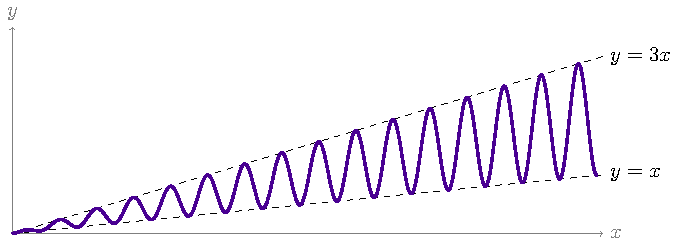
\includegraphics{fig/xsin(x+2).pdf}}

\end{QuestionSet}
\end{frame}

%------------------------------------------------------

%why does M have to be positive?